\documentclass[a4paper,UTF8]{article}
\usepackage{ctex}
\usepackage[margin=1.25in]{geometry}
\usepackage{color}
\usepackage{graphicx}
\usepackage{amssymb}
\usepackage{amsmath}
\usepackage{amsthm}
\usepackage{enumerate}
\usepackage{bm}
\usepackage{hyperref}
\usepackage{pgfplots}
\usepackage{epsfig}
\usepackage{color}
\usepackage{tcolorbox}
\usepackage{mdframed}
\usepackage{lipsum}
\usepackage{framed}
\usepackage{setspace}
\usepackage{listings}
\usepackage{float} %设置图片浮动位置的宏包

\newmdtheoremenv{thm-box}{myThm}
\newmdtheoremenv{prop-box}{Proposition}
\newmdtheoremenv{def-box}{定义}

\setlength{\evensidemargin}{.25in}
\setlength{\textwidth}{6in}
\setlength{\topmargin}{-0.5in}
\setlength{\topmargin}{-0.5in}
% \setlength{\textheight}{9.5in}
%%%%%%%%%%%%%%%%%%此处用于设置页眉页脚%%%%%%%%%%%%%%%%%%
\usepackage{fancyhdr}                                
\usepackage{lastpage}                                           
\usepackage{layout}                                             
\footskip = 10pt 
\pagestyle{fancy}                    % 设置页眉  


%%%%%%%%%%%% 这里也填一下 %%%%%%%%%%%%%%%%%%                
\lhead{201300035}           
%%%%%%%%%%%% 这里也填一下 %%%%%%%%%%%%%%%%%% 

           
\chead{数字信号处理}                                                
% \rhead{第\thepage/\pageref{LastPage}页} 
\rhead{作业四}                                                                                               
\cfoot{\thepage}                                                
\renewcommand{\headrulewidth}{1pt}  			%页眉线宽,设为0可以去页眉线
\setlength{\skip\footins}{0.5cm}    			%脚注与正文的距离           
\renewcommand{\footrulewidth}{0pt}  			%页脚线宽,设为0可以去页脚线

\makeatletter 									%设置双线页眉                                        
\def\headrule{{\if@fancyplain\let\headrulewidth\plainheadrulewidth\fi%
		\hrule\@height 1.0pt \@width\headwidth\vskip1pt	%上面线为1pt粗  
		\hrule\@height 0.5pt\@width\headwidth  			%下面0.5pt粗            
		\vskip-2\headrulewidth\vskip-1pt}      			%两条线的距离1pt        
	\vspace{6mm}}     								%双线与下面正文之间的垂直间距              
\makeatother  

%%%%%%%%%%%%%%%%%%%%%%%%%%%%%%%%%%%%%%%%%%%%%%
\numberwithin{equation}{section}
%\usepackage[thmmarks, amsmath, thref]{ntheorem}
\newtheorem{myThm}{myThm}
\newtheorem*{myDef}{Definition}
\newtheorem*{mySol}{Solution}
\newtheorem*{myProof}{Proof}
\newtheorem*{myRemark}{备注}
\renewcommand{\tilde}{\widetilde}
\renewcommand{\hat}{\widehat}
\newcommand{\indep}{\rotatebox[origin=c]{90}{$\models$}}
\newcommand*\diff{\mathop{}\!{d}}
\setlength{\parindent}{0pt}
\usepackage{multirow}

\lstset{language=Matlab}%这条命令可以让LaTeX排版时将Matlab关键字突出显示
\lstset{
	breaklines,%这条命令可以让LaTeX自动将长的代码行换行排版
	basicstyle=\footnotesize\ttfamily, % Standardschrift
	backgroundcolor=\color[rgb]{0.95,0.95,0.95},
	keywordstyle=\color{blue},
	commentstyle=\color{cyan},
	tabsize=4,numbers=left,
	numberstyle=\tiny,
	frame=single,
	%numbers=left, % Ort der Zeilennummern
	numberstyle=\tiny, % Stil der Zeilennummern
	%stepnumber=2, % Abstand zwischen den Zeilennummern
	numbersep=5pt, % Abstand der Nummern zum Text
	tabsize=2, % Groesse von Tabs
	extendedchars=false, %
	breaklines=true, % Zeilen werden Umgebrochen
	keywordstyle=\color{red},%这一条命令可以解决代码跨页时, 章节标题, 页眉等汉字不显示的问题
	stringstyle=\color{white}\ttfamily, % Farbe der String
	showspaces=false, % Leerzeichen anzeigen ?
	showtabs=false, % Tabs anzeigen ?
	xleftmargin=17pt,
	framexleftmargin=17pt,
	framexrightmargin=5pt,
	framexbottommargin=4pt,
	%backgroundcolor=\color{lightgray},
	showstringspaces=false % Leerzeichen in Strings anzeigen ?
}
\renewcommand{\lstlistingname}{CODE}
\lstloadlanguages{% Check Dokumentation for further languages ...
	%[Visual]Basic
	%Pascal
	%C
	Python
	%XML
	%HTML
	%Java
}


%--

%--
\begin{document}
	
	\title{数字信号处理\\
		作业四}
	\author{方盛俊\, 201300035} 
	\maketitle
	%%%%%%%% 注意: 使用XeLatex 编译可能会报错,请使用 pdfLaTex 编译 %%%%%%%
	
	\section*{作业提交注意事项}
	\begin{tcolorbox}
		\begin{enumerate}
			\item[(1)] 本次作业提交截止时间为~\textcolor{red}{\textbf{2022/12/18  23:59:59}},截止时间后不再接收作业,本次作业记零分;
			\item[(2)] 作业提交方式:使用此 \LaTeX 模板书写解答,只需提交编译生成的~pdf~文件,将~pdf~文件以 sftp 方式上传,账号为 dsp2022,密码为 12345asd!@。请远程连接 sftp://www.lamda.nju.edu.cn,提交到 /D:/courses/DSP2022/HW/HW4 路径下。
			\item[(3)] 文件命名方式:学号-姓名-作业号-v版本号, 例~ MG1900000-张三-4-v1;如果需要更改已提交的解答,请在截止时间之前提交新版本的解答,并将版本号加一;
			\item[(4)] 未按照要求提交作业,或~pdf~命名方式不正确,将会被扣除部分作业分数。
		\end{enumerate}
	\end{tcolorbox}
	
	
	\newpage
	\section{[60pts] 拉普拉斯变换}
	\begin{itemize}
		\item[1.]计算下列函数的拉普拉斯变换.
		\begin{itemize}
			\item[(1)]$ te^{-(t-2)}u(t-1) $
			\item[(2)]$ e^{-at}f\!\left(\frac{t}{a}\right) $, 已知 $\mathcal{L}[f(t)]=F(s)$
			\item[(3)]$ t^2\cos(2t) $
			\item[(4)]$ t^nu(t) $
			\item[(5)]$ f(t)=\left\{\begin{array}{ll}
				\sin (\omega t) & 0<t<\frac{T}{2},\ T=\frac{2 \pi}{\omega} \\
				0 & t \text { 为其他值 }
			\end{array} \right. $
		\end{itemize}
		
		\item[2.]求 $ \displaystyle \frac{4s+5}{s^2+5s+6} $ 的拉普拉斯反变换.
	\end{itemize}
	
	
	\begin{framed}
		\begin{spacing}{1.5}
			\begin{itemize}
        \item 1.

        (1)
        
        对于 $x(t) = te^{-(t-2)}u(t-1)$
        
        求拉普拉斯变换有
        
        $
        \begin{aligned}
        X(s) &= \int_{0^{-}}^{\infty}te^{-(t-2)}u(t-1)e^{-st}\mathrm{d}t  \\
        &= \int_{1^{-}}^{\infty}te^{-(t-2)}e^{-st}\mathrm{d}t  \\
        &= \frac{e^{2}}{(s+1)^{2}}\int_{1^{-}}^{\infty}(s+1)te^{-(s+1)t}\mathrm{d}(s+1)t  \\
        &= \frac{(- (s + 1)t - 1) e^{- (s + 1)t + 2}}{(s+1)^{2}}|_{1^{-}}^{\infty}  \\
        &= \frac{( s + 2 ) e^{- s + 1}}{(s+1)^{2}}  \\
        \end{aligned}
        $
        
        收敛域为 $\sigma > -1$.
        
        (2)
        
        对于 $\displaystyle x(t) = e^{-at}f(\frac{t}{a})$, 已知 $\mathcal{L}[f(t)] = F(s)$, 设 $f(t)$ 收敛域为 $\sigma > \sigma_0$.
        
        由展缩特性有 $\displaystyle \mathcal{L}[f(\frac{t}{a})] = aF(as)$, 收敛域变为 $\displaystyle \sigma > \frac{\sigma_0}{a}$.
        
        由指数加权和有 $\displaystyle X(s) = \mathcal{L}[e^{-at}f(\frac{t}{a})] = aF(a(s+a)) = aF(as+a^{2})$,
        
        收敛域为 $\displaystyle \sigma > \frac{\sigma_0}{a}-a$.
        
        (3)
        
        由于 $\displaystyle \mathcal{L}[\cos 2t] = \frac{s}{s^{2}+2^{2}} = \frac{s}{s^{2}+4}$,
        
        由线性加权特性可得
        
        $\displaystyle \mathcal{L}[t^{2}\cos(2t)] = \frac{\mathrm{d}^{2}\mathcal{L}[\cos 2t]}{\mathrm{d}s^{2}} = \frac{\mathrm{d}^{2}}{\mathrm{d}s^{2}}(\frac{s}{s^{2}+4}) = \frac{2 s (s^{2} - 12)}{(s^{2} + 4)^{3}}$
        
        收敛域为 $\displaystyle \sigma > 0$.
        
        (4)
        
        由于 $\displaystyle \mathcal{L}[u(t)] = \frac{1}{s}$,
        
        由线性加权特性可得
        
        $\displaystyle \mathcal{L}[t^{n}u(t)] = (-1)^{n} \cdot \frac{\mathrm{d}^{n}}{\mathrm{d}s^{n}}(\frac{1}{s}) = \frac{n!}{s^{n+1}}$
        
        收敛域为 $\displaystyle \sigma > 0$.
        
        (5)
        
        对于 $x(t) = \begin{cases}
            \sin(\omega t),  & 0 < t < \frac{T}{2}, T = \frac{2\pi}{\omega} \\
            0,  & \text{otherwise}
        \end{cases}$
        
        求拉普拉斯变换有
        
        $
        \begin{aligned}
        X(s) &= \int_{0^{-}}^{\infty}x(t)e^{-st}\mathrm{d}t  \\
        &= \int_{0^{-}}^{\frac{T}{2}}\sin(\omega t)e^{-st}\mathrm{d}t  \\
        &= \int_{0^{-}}^{\frac{\pi}{\omega}}\frac{e^{j\omega t}-e^{-j\omega t}}{2j}e^{-st}\mathrm{d}t  \\
        &= \frac{1}{2j(s-j\omega)}\int_{0^{-}}^{\frac{\pi}{\omega}}e^{-(s-j\omega)t}\mathrm{d}(s-j\omega)t  \\
        &\quad\  - \frac{1}{2j(s+j\omega)}\int_{0^{-}}^{\frac{\pi}{\omega}}e^{-(s+j\omega)t}\mathrm{d}(s+j\omega)t  \\
        &= \frac{-e^{-(s-j\omega)t}}{2j(s-j\omega)}|_{0^{-}}^{\frac{\pi}{\omega}} - \frac{-e^{-(s+j\omega)t}}{2j(s+j\omega)}|_{0^{-}}^{\frac{\pi}{\omega}}  \\
        &= (\frac{-e^{-(s-j\omega)\frac{\pi}{\omega}}}{2j(s-j\omega)} - \frac{-1}{2j(s-j\omega)}) - (\frac{-e^{-(s+j\omega)\frac{\pi}{\omega}}}{2j(s+j\omega)} - \frac{-1}{2j(s+j\omega)})  \\
        &= \frac{\omega (1 + e^{- \frac{\pi s}{\omega}})}{\omega^{2} + s^{2}}  \\
        \end{aligned}
        $
        
        收敛域为 $\sigma > -\infty$.
        
        \item 2.
        
        进行部分分式展开:
        
        $\displaystyle X(s) = \frac{4s+5}{s^{2}+5s+6} = \frac{4s+5}{(s+2)(s+3)} = \frac{k_1}{s + 2} + \frac{k_2}{s + 3}$
        
        其中
        
        $\displaystyle k_1 = (s+2)X(s)|_{s=-2} = \frac{4s+5}{s+3}|_{s=-2} = -3$
        
        $\displaystyle k_2 = (s+3)X(s)|_{s=-3} = \frac{4s+5}{s+2}|_{s=-3} = 7$
        
        即有 $\displaystyle X(s) = -\frac{3}{s+2} + \frac{7}{s+3}$
        
        进行拉普拉斯反变换可得
        
        $\displaystyle x(t) = -3e^{-2t}u(t) + 7e^{-3t}u(t)$
			\end{itemize}
		\end{spacing}
	\end{framed}
	
	
	
	
	\newpage
	\section{[40pts] 拉普拉斯变换的应用}
	已知一连续时间 LTI 系统的零状态响应
	$$
	y(t)=\left(1+0.6e^{-20t}-1.6e^{-10t}\right) x(t)
	$$
	已知 $x(t)=u(t)$, 由 $s$ 域求解:
	\begin{itemize}
		\item[(1)]该系统的系统函数 $H(s)$ 并画出零极点分布图;
		\item[(2)]写出描述系统的微分方程和系统, 并求 $h(t)$;
		\item[(3)]判断系统是否因果稳定.
	\end{itemize}
	
  \begin{framed}
    \begin{spacing}{1.5}
      \begin{itemize}

        \item (1)

        由 $x(t) = u(t)$ 可知
        
        零状态响应和激励信号的拉普拉斯变换分别为
        
        $\displaystyle Y_{zs}(s) = \frac{1}{s} - \frac{1.6}{s+10} + \frac{0.6}{s+20} = \frac{4 (s + 50)}{s (s + 10) (s + 20)}, \quad \operatorname{Re}(s) > 0$
        
        $\displaystyle X(s) = \frac{1}{s}, \quad \operatorname{Re}(s) > 0$
        
        因此有系统函数
        
        $\displaystyle H(s) = \frac{Y_{sz}(s)}{X(s)} = \frac{4 (s + 50)}{(s + 10) (s + 20)} = \frac{4 s + 200}{s^{2} + 30 s + 200}, \quad \operatorname{Re}(s) > -10$
        
        对应的零极点分布图为
        
        \begin{figure}[H]
          \centering
          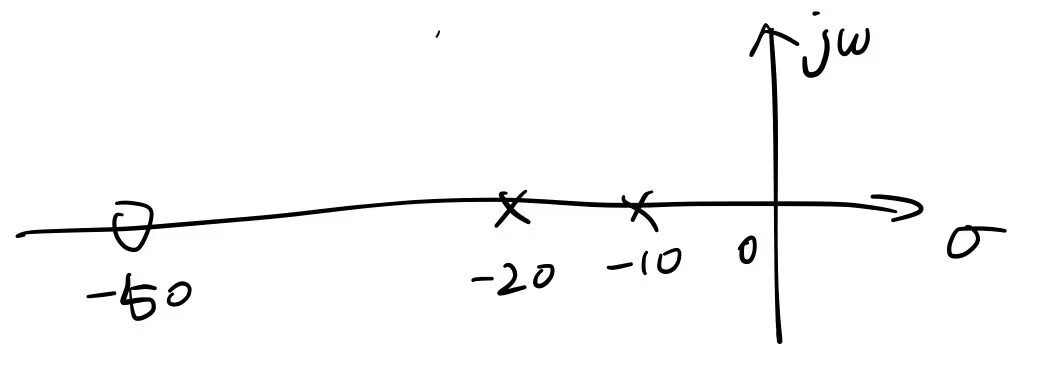
\includegraphics[width=0.9\textwidth]{images/2022-12-12-12-52-26.png}
          \label{Fig.main1}
        \end{figure}
        
        \item (2)
        
        由系统函数
        
        $\displaystyle H(s) = \frac{Y_{sz}(s)}{X(s)} = \frac{4 (s + 50)}{(s + 10) (s + 20)} = \frac{4 s + 200}{s^{2} + 30 s + 200}, \quad \operatorname{Re}(s) > -10$
        
        可得
        
        $\displaystyle (s^{2} + 30 s + 200)Y_{zs}(s) = (4s + 200)X(s)$
        
        两边进行拉普拉斯反变换, 可得描述系统的微分方程为
        
        $\displaystyle y''(t) + 30y'(t) + 200y(t) = 4x'(t) + 200x(t)$
        
        将系统函数进行部分分式展开有
        
        $\displaystyle H(s) = \frac{Y_{sz}(s)}{X(s)} = \frac{4 (s + 50)}{(s + 10) (s + 20)} = \frac{k_1}{s + 10} + \frac{k_2}{s + 20}$
        
        其中
        
        $\displaystyle k_1 = (s+10)H(s)|_{s=-10} = \frac{4(s+50)}{s+20}|_{s=-10} = 16$
        
        $\displaystyle k_2 = (s+20)H(s)|_{s=-20} = \frac{4(s+50)}{s+10}|_{s=-20} = -12$
        
        因此我们有
        
        $\displaystyle H(s) = \frac{Y_{sz}(s)}{X(s)} = \frac{4 (s + 50)}{(s + 10) (s + 20)} = \frac{16}{s + 10} - \frac{12}{s + 20}$
        
        再进行拉普拉斯反变换, 可得系统冲击响应为
        
        $\displaystyle h(t) = (16e^{-10t} - 12e^{-20t})u(t)$
        
        \item (3)
        
        系统冲击响应 $\displaystyle h(t) = (16e^{-10t} - 12e^{-20t})u(t)$,
        
        满足 $h(t) = 0, t < 0$, 因此系统为因果系统.
        
        由 (1) 中零极点分布图可以看出, 系统的极点位于 $s$ 左半平面, 因此系统稳定.
        
        
      \end{itemize}
    \end{spacing}
  \end{framed}
	
\end{document}